% !TeX program = xelatex
\documentclass[UTF8,a4paper,11pt,fontset=none]{ctexart}
\usepackage[margin=22mm,headheight=16pt]{geometry}
\usepackage{fontspec,amsmath,amssymb,graphicx,booktabs,tabularx,array,xcolor,fancyhdr,enumitem}
\usepackage[colorlinks=true,linkcolor=navy,urlcolor=teal,citecolor=teal]{hyperref}
\setmainfont{Times New Roman}
\setsansfont{Arial}
\setmonofont{Menlo}[Scale=0.82]
\setCJKmainfont{Songti SC}[BoldFont=Heiti SC]
\setCJKsansfont{Heiti SC}
\setCJKmonofont{Heiti SC}
\definecolor{navy}{HTML}{164D6B}
\definecolor{teal}{HTML}{247C80}
\definecolor{muted}{HTML}{617282}
\definecolor{pendingred}{HTML}{B12D36}
\definecolor{pale}{HTML}{EFF4F7}
\hypersetup{pdftitle={雷达—视觉未来占据预测：阶段工作报告},pdfauthor={RadarFlowOcc Research},pdfsubject={2026年9月14日至17日研究进展与实验决策}}
\ctexset{section={format=\Large\bfseries\color{navy}},subsection={format=\normalsize\bfseries\color{navy}}}
\setlength{\parindent}{2em}
\setlength{\parskip}{4pt}
\linespread{1.13}
\setlist{nosep,leftmargin=1.7em,topsep=4pt}
\renewcommand{\arraystretch}{1.2}
\newcolumntype{Y}{>{\raggedright\arraybackslash}X}
\newcommand{\pending}[1]{\textcolor{pendingred}{#1}}
\newcommand{\evidence}[1]{{\footnotesize\color{muted}\par\noindent 证据索引：#1。\par}}
\newcommand{\takeaway}[1]{\par\noindent\colorbox{pale}{\parbox{\dimexpr\linewidth-2\fboxsep}{\vspace{3pt}\textbf{阶段判断}\quad #1\vspace{3pt}}}\par}
\pagestyle{fancy}\fancyhf{}
\fancyhead[L]{\small\color{muted}RadarFlowOcc\quad 研究工作报告}
\fancyhead[R]{\small\color{muted}2026.09.17}
\fancyfoot[L]{\footnotesize\color{muted}内部研究记录 · 单种子证据 · 未作为论文定稿}
\fancyfoot[R]{\small\thepage}
\renewcommand{\headrulewidth}{0.3pt}
% Values generated from independently audited completed D artifacts.
\newcommand{\DCurrent}{14.2910}
\newcommand{\DFuture}{8.2462}
\newcommand{\DMoving}{21.2271}
\newcommand{\DStationary}{48.4989}
\newcommand{\DArrival}{2.3381}
\newcommand{\DVacating}{8.4248}
\newcommand{\DOverview}{D 的完整结果也已取回并通过独立复算，未来 GMO 为8.2462\%，本轮三臂均未达到目标。}
\newcommand{\DInterpretation}{D 为8.2462\%，比自身保持低1.3537个百分点，95\%场景区间[$-1.7133,-1.0265$]。三臂均不支持扩大为全验证或少帧训练候选。}
\newcommand{\StatusParagraph}{2026年9月17日20:42（北京时间）只读检查确认，T/J/D服务器序列正常退出，D训练完成2,048次更新、评价完成；T最终权重train512评价亦完成。随后取回D的全部小型文本结果，核验文件哈希、训练顺序、原O指标与GT有效域，并独立复算796项聚合标量和同源物理参考。少帧实验尚未启动。}

\begin{document}
\thispagestyle{empty}
\noindent{\sffamily\color{teal}\small RESEARCH PROGRESS REPORT\hfill 2026 / 09 / 17}\par
\vspace{9mm}
\noindent{\LARGE\bfseries\color{navy}雷达—视觉未来占据预测}\par
\vspace{2mm}
\noindent{\Large 阶段工作报告：从运动连接诊断到视觉历史替代}\par
\vspace{4mm}
\noindent\textcolor{muted}{覆盖阶段：2026年9月14日至17日\quad 研究目标：面向 ICLR 的可验证方法贡献}
\vspace{5mm}

\takeaway{已建立可复用的强对照 O，并完成多轮运动信息、任务连接和状态传播诊断。当前新候选尚未同时实现“超过 O”与“运动预测更准确”。下一重点是验证 Doppler 动态观测能否减少视觉历史需求，并形成真实的性能—计算优势。}

\section*{本阶段的主要进展}
\begin{enumerate}
\item \textbf{保留一个已验证的性能改进。} 在相同原生评价协议的5,119个验证锚点上，O 的未来 GMO IoU 为14.7478\%，匹配精度的 M0 为13.9449\%，提升0.8029个百分点。该结果确立强对照，但不能证明运动机制已改善。
\item \textbf{将占据收益与运动收益分开核验。} 若干连接或残差候选提高总体 IoU，却降低运动目标召回；对象速度置换、置零实验显示，输入中含速度不等于预测真正利用速度。
\item \textbf{完成冻结视觉运动证据与状态原型诊断。} 更密集的历史改善 DELTA 的运动估计，但仍未超过现有 CV+D 对照。小样本上可拟合的内容传播原型扩大到 train512 后，T/J 的 dev200 结果均明显低于 O。\DOverview
\item \textbf{识别训练拟合阶段的问题。} 固定 T 最终权重，在其训练集上重新评价得到未来 GMO 10.8284\%，低于自身当前输出保持的11.3461\%；不能仅将开发集失败归因于泛化。
\item \textbf{提出可检验的效率贡献。} 以真实相机时间点 H=1/3 和三种传感器条件构成首轮六组对照；目前完成计划与输入审计，\pending{尚无少帧性能或端到端加速结论}。
\end{enumerate}

\section*{统一任务与证据口径}
输入为当前及历史相机、雷达观测，以及原协议允许的未来自车条件；预测0.5、1.0、1.5、2.0秒的体素占据。GMO 是\textbf{可移动语义集合}，其中包含当时静止的车辆等对象，不等于“正在运动”。主指标为各未来时域先池化混淆矩阵，再平均正类 IoU：
\[
 Q_{\mathrm{future}}=\frac{1}{4}\sum_{h=1}^{4}
 \frac{\mathrm{TP}_h}{\mathrm{TP}_h+\mathrm{FP}_h+\mathrm{FN}_h}.
\]
它不是语义 mIoU，也不是两个类别的平均 IoU，不能直接与其他论文标题相似、口径不同的30\%数值比较。本报告所有数值图均来自真实结果；缺项使用红字标记，不生成模拟结果。

\clearpage
\section{强对照 O：优化目标修订与完整评价}
\subsection{实际改进与可复用资产}
O 从原始 M0 初始化，冻结图像与雷达观测主干，只训练完整未来预测头。其目标保留原类别加权交叉熵与 Lov\'asz，semantic/geometric scaling 项仍做有限值检查，但不参与优化。这里移除的是特定辅助目标，\textbf{不是移除全部监督，也不是证明物理或运动监督无用}。

训练使用512个锚点、256个场景，单 seed11，四轮共2,048次样本使用，梯度累积4，对应512次 AdamW 更新。匹配控制 C 保留原训练目标。O 资产由“M0 完整模型 + O 的完整未来预测头”组成；预测头含13,274,016个参数，不能把它当作独立完整模型权重。

\begin{center}
\small
\begin{tabular}{lrr}
\toprule
完整原生验证：5,119 anchors / 150 scenes & 未来 GMO / \% & 相对匹配对照 / pp\\
\midrule
M0（匹配 future matmul 精度） & 13.9449 & ---\\
C（匹配训练控制） & 13.7276 & ---\\
O（保留模型） & \textbf{14.7478} & O$-$M0：+0.8029\\
\bottomrule
\end{tabular}
\end{center}
\begin{center}
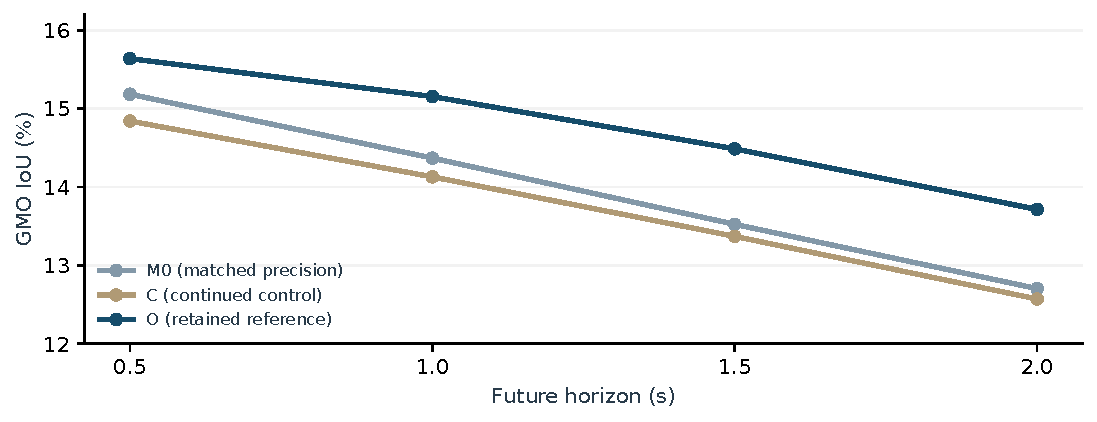
\includegraphics[width=.94\linewidth]{figures/full5119_horizons.pdf}
\par\small 图1：相同5,119个样本的真实未来 GMO 曲线。仅连接已测时域。
\end{center}

O$-$M0 的场景配对 bootstrap 95\%区间为[+0.6818,+0.9406]个百分点；O$-$C 为+1.0202个百分点，区间[+0.9296,+1.1115]。重采样以场景为单位、重复10,000次，\textbf{描述场景抽样变化，不覆盖训练种子或模型选择的不确定性}。

\subsection{对 loss 移除的研究解释}
当前证据支持：在既定表示、标签、训练预算和读出方式下，简化目标改善了任务指标。它尚未区分损失尺度、梯度方向、类别偏置和读出校准等原因，不能把“优化干扰”写成已确定的唯一原因。

相对 C，O 四未来时域的 FP 总计减少约9,671万，但 FN 增加约828万。相对 M0，整体 FP/FN 减少，但较远两个时域 FN 上升；当前时刻 GMO 还下降0.1396个百分点。因此下一阶段必须同时检查 moving recall、静止误运动和到达/离开占据，避免用抑制前景预测换取单一 IoU 提升。
\evidence{E1：O 模型卡、完整评价 CSV 与独立审查；原验证集存在历史曝光，不称全新盲测}

\clearpage
\section{运动信息与任务连接：已排除的解释}
\subsection{连接成立，不代表动态信息有效}
早期 R/R0 未来特征残差对照，在 dev200 上分别为15.2012\%和15.2367\%，却都低于 O 的运动目标召回；R$-$R0 的差异区间跨零。早期 connected-motion J/D、未来状态监督 K/B 和对象状态 V/G 同样没有建立实用的运动增益。这些名称属于不同实验族；\textbf{本报告第3节的 dense-material T/J/D 是新的独立实验，不与早期同字母结果混用}。

对同一最终 V 权重，将对象速度正确输入、帧内交换或置零，未来 GMO 均约14.8768\%，2秒 moving XY EPE 均约4.20543 m。输入速度确实发生变化，而终端指标近乎不变。这表明该模型终点缺乏有效的速度利用；不说明雷达测速本身没有信息。

\subsection{冻结 RAFT：证据评分尚不胜过简单速度先验}
完成 train512/256场景的9,216次官方 RAFT 前向，零优化更新。在无同格雷达回波、CRN 未覆盖的共同图像有效点集上，2秒运动收益排序 AUC 为：RAFT 0.5096、打乱历史0.4967、预测速度0.6008。440项 AUC 独立复算最大差为$2.22\times10^{-16}$。该 AUC 衡量位移方案是否更有利，\textbf{不是未来占据 IoU，也不是光流准确率}。

高预测速度子集出现更强信号，但覆盖和负例对象权重不足以建立全局门控。源点还是 GT 框定义的虚拟材料点，尚未认证为实际可见表面，因而不能直接作为可部署查询生成器。

\subsection{更强历史对应：多帧有帮助，但强对照仍胜出}
在相同 train16/8场景上，冻结 Metric3D 和官方 DELTA，将96条六相机序列由两帧增加为同起止时刻的5--7帧。各方案在 CRN 覆盖区域保留恒速外推，仅在覆盖外接入图像运动场。
\begin{center}\small
\begin{tabularx}{\linewidth}{Yrr}
\toprule
2秒 XY 位移 EPE（m，越低越好） & moving，137 & stationary，184\\
\midrule
CRN-CV & 3.0223 & \textbf{0.0922}\\
CV+D，固定0.5 m/s规则 & \textbf{2.7377} & 0.1010\\
CV+两帧 RAFT，FB筛选 & 3.2945 & 0.3903\\
CV+两帧 DELTA，官方可见性 & 2.9970 & 0.2669\\
CV+密集 DELTA，端点差分 & 2.8989 & 0.1887\\
CV+密集 DELTA，当前锚定 LSQ & 2.8937 & 0.1884\\
\bottomrule
\end{tabularx}\end{center}
这里分母是 anchor-instance，EPE 为对象等权的\textbf{XY 刚体框代理}，不能与后文 XYZ 直接横比。各质量掩码不同，原对象分母及回退仍保留。密集历史的改善也出现在不筛选的比较中，但不能归因于单一机制；这些实验没有产生新的 O 占据收益。
\takeaway{停止继续扩展当前“外部深度/跟踪器 $\rightarrow$ 确定三维速度 $\rightarrow$ 恒速外推”的路线。保留冻结输出与 CV+D，下一步检验运动信息怎样进入可被任务使用的状态。}
\evidence{E2：R/R0 与速度分配诊断；E3：冻结 RAFT；E4：密集 DELTA 与独立几何/评分核验}

\clearpage
\section{状态传播原型：扩大数据后的真实结果}
\subsection{实验设计与小样本发现}
先用同一 encoder/decoder 检验内容与运动的作用：T 用固定当前内容进行传播；J 用演化内容进行传播；D 直接读出演化状态，占据路径不依赖位移。T 的递推状态仍参与位移生成，并非把整个内容分支冻结。三臂共享当前 codec、初始参数、样本顺序和训练预算。

train4 诊断中，T/J 的未来 IoU 为21.2815\%/20.8018\%，moving 2秒 EPE 为1.1163/2.2045 m；它只说明极小数据上的可拟合性。随后固定数值策略，在 train512/256场景上训练共同当前 codec，三臂各2,048次更新。

\subsection{dev200：同一原任务、同一评价人口}
\begin{center}\small
\begin{tabular}{lrrrr}
\toprule
指标 & O & T & J & D\\
\midrule
当前 GMO / \% & 15.9191 & 14.2910 & 14.2910 & \DCurrent\\
未来 GMO / \% & 14.6640 & 9.2876 & 9.0291 & \DFuture\\
moving recall / \% & 43.4521 & 30.2357 & 26.7237 & \DMoving\\
stationary recall / \% & 47.4253 & 42.1910 & 46.6085 & \DStationary\\
到达 01 IoU / \% & 8.1234 & 3.7572 & 3.0122 & \DArrival\\
离开 10 IoU / \% & 9.9818 & 8.4546 & 7.7217 & \DVacating\\
\bottomrule
\end{tabular}\end{center}
\noindent\small 所有数值来自相同200个开发锚点/100场景。moving 为速度$>0.5$ m/s，stationary 为$\leq0.1$ m/s；中间组保留为 ambiguous。\normalsize

\begin{center}
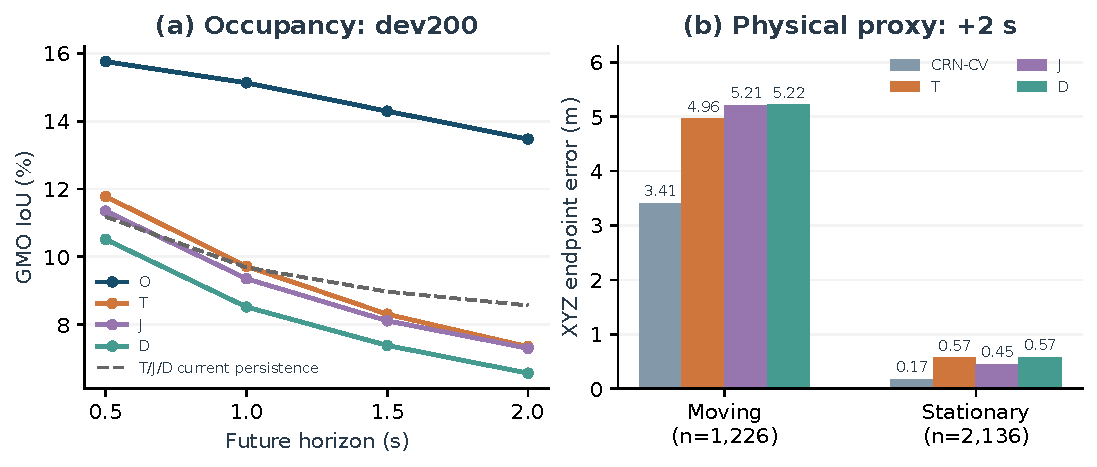
\includegraphics[width=.94\linewidth]{figures/dev200_comparison.pdf}
\par\small 图2：真实开发集结果。左：原任务 GMO。右：名义2秒 XYZ 框代理 EPE；O 无认证物理运动头，因此不填 O 的 EPE。
\end{center}

T/J 自身当前保持的未来 GMO 均为9.5999\%；T$-$保持为$-0.3122$个百分点，场景95\%区间[$-0.6378,+0.0490$]，J$-$保持为$-0.5708$，区间[$-0.8866,-0.2461$]。J 内容会演化，保持当前输出\textbf{不等于} J 的零位移干预。\DInterpretation

\textbf{与 O 的比较边界：}原型只使用缓存当前 BEV，训练52,720个参数；O 保留完整未来头及协议允许的 future ego/action/query 条件。原型与 O 的差距说明候选整体失败，不是控制单模块后的因果效应；更新数相同也不意味着计算预算相同。

\clearpage
\section{T 的最终权重诊断：问题已出现在训练集}
\subsection{为何补做固定权重 train512 评价}
开发集失败可能来自训练拟合不足、状态信息不足、读出不匹配或泛化。为先区分“训练上就未学好”与“只在开发场景失效”，使用 T 同一最终 checkpoint，对原512个训练锚点做完整细粒度评价；\textbf{没有新增优化更新、调参或挑选 checkpoint}。

\begin{center}\small
\begin{tabular}{lrrr}
\toprule
评价人口 & 当前 GMO / \% & 未来 GMO / \% & 当前保持 / \%\\
\midrule
train512 / 256 scenes & 16.5057 & 10.8284 & 11.3461\\
dev200 / 100 scenes & 14.2910 & 9.2876 & 9.5999\\
\bottomrule
\end{tabular}\end{center}
\begin{center}
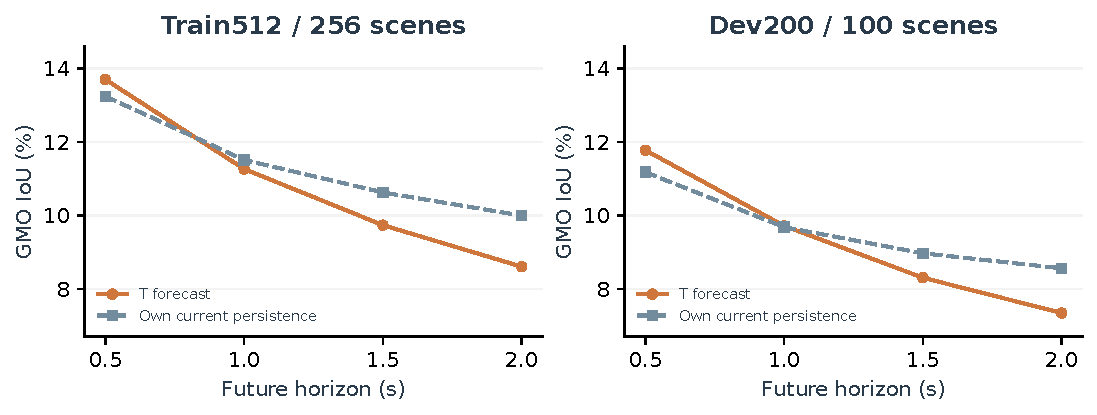
\includegraphics[width=\linewidth]{figures/T_fit_diagnosis.pdf}
\par\small 图3：固定 T 最终权重的真实逐时域结果。训练集和开发集各自在相同有效域上比较预测与自身当前保持，不跨人口解释分差。
\end{center}

T 在训练集的未来平均分数比自身保持低0.5176个百分点；0.5秒略优，随后三个时域变差。训练集当前 GMO 16.5057\%不能与 O 的验证集未来分数比较。训练集2秒 moving XYZ EPE 为4.8458 m，stationary 为0.4851 m；本次没有建立 O 的训练集物理参考。

独立审计核验了输入、标签、最终权重身份及120,042个分类标量，确认保持对照与预测采用同一未来有效域。该检查验证统计与来源；并不替代一次独立网络重跑。

\subsection{目前可以支持的研究解释}
\begin{enumerate}
\item \textbf{失败不只是开发集泛化问题。} 训练集终点已经低于保持当前输出，优先检查预测目标与状态读出的关系，而不是直接扩大验证或训练种子数。
\item \textbf{当前重建能力不等于动态充分性。} 共同 codec 只接受当前占据监督；它能读出当前形状，不代表保留了未来所需的运动、遮挡和身份信息。也不能反过来断言这些信息已被不可逆地抹去。
\item \textbf{运动代理和占据预测是两条证据线。} 比零位移更低的 EPE 并不足够；仍需超过 CRN-CV 等强参考，并改善全域占据和 moving recall。
\item \textbf{避免过度归因。} 当前结果未证明训练已收敛，未证明缺少 future ego/action 是唯一原因，也未否定所有 latent transport。名义0.5秒积分与真实采集间隔亦需在后续方法中明确处理。
\end{enumerate}
\takeaway{停止扩大当前 T/J/D 候选；本轮内容/传播诊断已完成。下一模型需要保留 O 已有预测能力，并证明新增动态信息改变了任务输出。}
\evidence{E6：固定 T 的 train512 完成回执与独立统计，零优化更新}

\clearpage
\section{文献与仓库调研如何改变研究判断}
近期调研覆盖世界模型、三维跟踪、持久状态和运动驱动读出；工作分为论文筛选、方法阅读、固定提交源码核验和冻结权重运行。\textbf{看过论文或仓库不等于完成复现，以下迁移判断仍是研究推论。}

\begin{center}\small
\begin{tabularx}{\linewidth}{p{31mm}YY}
\toprule
参考方向 & 已明确的借鉴点 & 对本项目的适用边界\\
\midrule
Drive-HWM\cite{hwm} & 用动态相关目标学习未来隐表示，连接到行动预测 & NAVSIM 驾驶结果不能代替本项目的未来占据与物理 EPE；不因此直接增加光流 loss\\
低秩动态载体\cite{carrier} & 区分“可读出运动”和“干预后自主未来改变”，加入目标特异性控制 & 简化双对象环境；低秩入口不是封闭低维动力学，也不是道路场景反事实真值\\
DriveCache\cite{cache} & 评价局部计算复用对终端输出的后果，考虑自车平移/转弯 & 缓存扩散去噪步，不能把四个物理预测时域当作等价去噪步\\
JEPA-WMs\cite{jepa} & 分开预测状态、独立读出探针和终端任务；核对多步 rollout 训练 & 机器人规划中的 embedding 误差或 decoder 结果不是本项目占据收益\\
DELTA\cite{delta} & 真实相机标定、时序对应与共同坐标系；已运行官方冻结权重 & 更密历史提高估计，但本项目强对照仍更好；跟踪已观测视频不等于预测未来\\
CRISP / TEOcc\cite{crisp,teocc} & 雷达、Doppler、时序融合与未来表示已有近邻先例 & 不能主张“首次将雷达用于动态世界建模”；须证明历史替代与实际成本收益\\
\bottomrule
\end{tabularx}\end{center}

\subsection{从“再加模块”转为三个可证伪问题}
\textbf{信息：} 合法的雷达动态量测与相机历史，是否提供超过几何、速度幅值和覆盖先验的额外信息？应以同点、同时间、同有效域及错配控制回答，不能靠删除困难样本改善分数。

\textbf{连接：} 改变正确目标的运动信息，是否选择性地改变该目标的未来占据？需要真实前向干预、目标/非目标区域响应和最终标签评价；非零梯度仅证明计算连接，不能证明有用。

\textbf{效用：} 信息与连接成立后，是否改善完整场景的准确性或性能—计算曲线？小样本重建、代理 EPE 和低秩读出都不能独立完成这一步。

\subsection{新颖性应收窄到可量化的替代关系}
CRISP 已明确将雷达 range/Doppler 用于 BEV 时间传播及预测预训练，当前公开条目标注 under review\cite{crisp}。因此本项目更有辨识度的候选问题是：\textbf{在严格记录两种传感器历史预算时，直接动态观测能够替代多少视觉历史，在哪些可观测条件下成立？}

\evidence{E7：三篇指定论文笔记、世界模型综合调研、JEPA-WMs 与 CRISP 专项源码/正文审查；正文引文指向原始来源}

\clearpage
\section{新增主线：用 Doppler 减少视觉历史与计算}
\subsection{科学假设与物理边界}
视觉序列可通过对应关系推断位移和速度；Doppler 直接约束视线方向的相对运动。完成自车运动补偿后，一个简化观测关系为
\[
 z_i^{\mathrm{comp}}=\mathbf u_i^\top\mathbf v+\epsilon_i,
\]
其中$\mathbf u_i$为视线单位方向。它约束一个速度分量；切向运动、身份关联、遮挡恢复和未来行为仍可能依赖视觉或先验。因此假设是\textbf{部分替代视觉历史}，不是雷达完整测得三维动态。

\takeaway{待验证命题：短历史相机 + 雷达 Doppler，在相同任务与质量门槛下，可达到长历史纯视觉的预测水平，并减少真实端到端成本。当前尚未证明。}

\subsection{已完成的输入审计}
原生 O 以两个历史时刻加当前时刻作为输入（队列参数为2），即 H=3，每时刻六相机，共18张图像；其 memory queue 长度为1，仅表示最终 BEV 槽数。当前缓存已经融合历史，不能截取一个槽就称 H=1。

原雷达为五传感器、每路至多五 sweeps，含补偿速度及派生通道。实际反例发现：将 \texttt{nsweeps} 从5改为1仍读取同一个旧缓存。必须建立绑定输入配置的新缓存，才能认证单 sweep 对照。训练与开发锚点全部具备八时刻 sample 链，但这不等于各 H 的图像文件与传感器时间戳均已认证。

H1/H2/H3 窗口选择模块与真实前向 probe 源码已编写；\pending{尚无本报告可引用的真实 H1 模型前向通过回执}。少帧模块不能因语法或局部接口检查通过就写成运行完成。

\subsection{首轮六组实验与决定性比较}
\begin{center}\small
\begin{tabularx}{\linewidth}{lYY}
\toprule
输入条件 & H=1：一个多视角时刻 & H=3：三个多视角时刻\\
\midrule
camera-only & \pending{待训练与评价} & \pending{待匹配训练与评价}\\
camera + radar geometry/RCS & \pending{待训练与评价} & \pending{待训练与评价}\\
camera + geometry/RCS + Doppler & \pending{待训练与评价} & \pending{待训练与评价}\\
\bottomrule
\end{tabularx}\end{center}
共享自有 backbone、解码器、初始化、场景、未来标签、分辨率及单 seed11。主比较固定雷达观测窗口，并完整移除 Doppler 及其派生/预处理泄漏；第三方 baseline 仍只用官方权重。测试时截短历史的诊断与按短历史适配训练的主结果分别报告。

定义同 H 的动态增益 $D(H)=Q(C+R_{\rm geom}+R_{\rm dop},H)-Q(C+R_{\rm geom},H)$。检查短历史是否更受益，并比较短历史完整模型与长历史纯视觉。\textbf{正式跑前}冻结质量非劣界限、成本改善门槛和确认场景；目前阈值尚未冻结。

\textbf{成本必须实测：}同时报告图像/雷达编码、时间融合、rollout、预处理和总延迟的 median/p95、显存及 FLOPs。区分窗口重算与真正 streaming；复用历史特征时，减少 H 未必按比例减少每步图像编码。缓存 BEV 的训练耗时不能代替端到端速度证据。

\clearpage
\section{下一阶段安排、停止条件与证据归档}
\begin{center}\small
\begin{tabularx}{\linewidth}{p{22mm}YY}
\toprule
阶段 & 交付与通过条件 & 不通过时的动作\\
\midrule
结束当前诊断 & 完整 T/J/D、T 训练集结果与同源统计归档；区分状态不足和读出不足的证据 & 不扩大失败候选到完整验证，不追加多种子\\
合法输入验证 & H3 包装与原生输出等价；H1 只改变观测窗口；当前图像、未来 GT、自车条件不变；新 radar 缓存可追溯 & 修复输入/任务耦合，不用旧融合缓存冒充少帧\\
单种子六组比较 & 冻结质量/成本门槛，比较 C、几何和 Doppler；占据与 moving/stationary 同报 & 若仅同 H 融合有收益，限制结论；不宣称视觉历史替代\\
机制与成本确认 & Doppler 移除/错配、径向/切向、距离与遮挡分组；端到端与 streaming 测量 & 若只冷启动提速，则仅报告窗口/启动收益\\
场景确认与写作 & 路线冻结后在场景分离人口确认；统一任务对照、消融、成本和失败案例 & 若无法重复实用收益，转向任务连接或传感器退化可靠性问题\\
\bottomrule
\end{tabularx}\end{center}

\subsection{面向 ICLR 尚缺的核心证据}
现阶段已有强对照、可追溯的失败诊断和新的可证伪假设，但\pending{尚无经过确认的主方法贡献}。论文需要补齐：同任务强对照上的实用收益；Doppler 的独立作用；变化确实进入未来预测；成本优势；适用与失败条件。单数据集、单训练种子仍是明确限制，不以场景 bootstrap 替代种子稳定性。遵循节约时间的要求，当前不安排多种子。

原验证集排除 dev200 所属100个场景后，已记录50场景/1,707锚点的场景分离确认人口，与 train512 场景不相交。但完整验证集有既往使用，\textbf{不能称从未曝光的新盲测}。正式发表所需的更强独立性或跨条件证据仍需规划。

\subsection{当前执行状态与保存范围}
\StatusParagraph
报告没有启动新训练、停止既有作业或修改 O/M0；旧 S3 不恢复。所有缺失结果以红字标记。源码、协议、小型聚合结果及报告纳入 GitHub；权重、数据集、原始大数组和连接配置保留在原环境。

\subsection{复核索引}
下列索引对应工作区证据。随包证据清单记录文件路径与 SHA256；\texttt{data.json} 保存绘图所用真实聚合值。
\begin{description}[style=nextline,font=\bfseries\small,itemsep=1pt]
\item[E1] \small \texttt{m0\_improvement\_20260915}：O模型卡、完整共同评价 CSV。
\item[E2--E4] \small \texttt{o\_motion\_20260915}：R/R0、速度分配、冻结RAFT、密集DELTA结果与审计。
\item[E5--E6] \small \texttt{dense\_material512\_*\_evidence\_v1.json}；\texttt{material512\_train\_fit\_evidence\_v1.json}；训练与评价完成回执。
\item[E7--E8] \small \texttt{research\_notes/} 文献/源码记录；视觉历史输入审计、缓存反例、少帧实验计划。
\end{description}

\clearpage
\section*{参考文献与报告复现说明}
文献状态按2026年9月17日可核对的原始页面记录。会议论文与预印本分开标注；文献方法的成功不作为本项目成功证据。
\begin{thebibliography}{9}\small
\bibitem{hwm} Z. Fan et al. \emph{Drive-HWM: Hierarchical World Models for Dynamic-Latent Guided Autonomous Driving}. arXiv:2609.03572v1, 2026（预印本）. \url{https://arxiv.org/abs/2609.03572}.
\bibitem{carrier} Y. Liu and Y. Chen. \emph{Low-Rank Dynamics-Effective Latent Carriers for Counterfactual Rollout in Learned World Models}. arXiv:2608.15156v4, 2026（预印本）. \url{https://arxiv.org/abs/2608.15156}.
\bibitem{cache} J. Yang et al. \emph{DriveCache: Action-Aware Caching for Driving World Model Inference}. arXiv:2608.16354v1, 2026（预印本）. \url{https://arxiv.org/abs/2608.16354}.
\bibitem{jepa} B. Terver et al. \emph{What Drives Success in Physical Planning with Joint-Embedding Predictive World Models?} arXiv:2512.24497v4（页面记录 TMLR 接收）. \url{https://arxiv.org/abs/2512.24497}. 官方源码审查基于 \texttt{facebookresearch/jepa-wms} 的提交 \texttt{13cf1d9}，未运行该外部模型。
\bibitem{delta} \emph{DELTA: Dense Efficient Long-Range 3D Tracking for Any Video}. ICLR 2025. \href{https://proceedings.iclr.cc/paper_files/paper/2025/hash/6e1e1d2e58afe1007da0bb76fac722a0-Abstract-Conference.html}{ICLR正式论文页}. 本项目冻结运行的官方仓库：\url{https://github.com/snap-research/DELTA_densetrack3d}，提交 \texttt{3367cda}。
\bibitem{crisp} J. Song, Y. Liu, and K. A. Skinner. \emph{CRISP: A Spatiotemporal Camera-Radar Backbone for Driving via Forecasting-Based World-Model Pretraining}. arXiv:2607.04541v1, 2026（页面标注 under review）. \url{https://arxiv.org/abs/2607.04541}.
\bibitem{teocc} \emph{TEOcc: Radar-camera Multi-modal Occupancy Prediction via Temporal Enhancement}. ECAI 2024；官方实现与论文入口：\url{https://github.com/VDIGPKU/TEOcc}.
\end{thebibliography}

\subsection*{文件包}
\begin{itemize}
\item \texttt{main.tex}：可编辑中文 LaTeX 正文；\texttt{latest\_results.tex}：本次核实状态及 D 结果。
\item \texttt{main.pdf}：编译后的报告；\texttt{figures/}：三张矢量 PDF 与 PNG 预览。
\item \texttt{data.json}、\texttt{evidence\_manifest.json}：数值与来源身份；不包含模型权重和原始传感器数据。
\item \texttt{make\_figures.py}：从随包真实数据重绘图；\texttt{build.sh}：两遍 XeLaTeX 编译。
\end{itemize}
本机使用 XeLaTeX、ctex 与 macOS Songti/Heiti 字体。跨平台编译可将 CJK 字体改为已安装的 Noto Serif/Sans CJK SC，或使用相应 ctex 字体配置。报告为阶段记录，后续更新应重新核对完成回执和聚合结果，不能仅替换状态文字。
\end{document}
